% FPGA Percolation Project — Beamer Presentation Draft
% Compile with: pdflatex presentation.tex (x2 for TOC)
\documentclass[aspectratio=169, 11pt]{beamer}

% ---- Theme ----
\usetheme{Berlin}
\usecolortheme{whale}
\setbeamertemplate{navigation symbols}{}
\setbeamertemplate{footline}[frame number]

% ---- Packages ----
\usepackage[utf8]{inputenc}
\usepackage[T1]{fontenc}
\usepackage{amsmath, amssymb}
\usepackage{graphicx}
\usepackage{booktabs}
\usepackage{hyperref}
\usepackage{microtype}
\usepackage{tikz}
\usepackage{bookmark}
\usetikzlibrary{shapes, arrows, arrows.meta, positioning, fit, calc}



% ---- Metadata ----
\title{FPGA Accelerator for Directed Percolation}
\subtitle{Monte Carlo Simulation on Artix-7 at 100 MHz}
\author{Leonardo Pieripolli, Alessio Tuscano}
\institute{Programmable Hardware Devices}
\date{\today}

% ---- Custom commands ----
\newcommand{\pc}{p_{\!c}}
\newcommand{\nup}{1/\nu}
\newcommand{\nud}{1/\nu_{\!\|}}

\graphicspath{{figures/}}

\begin{document}

% ============================================================
%  SLIDE 1 — Title
% ============================================================
\begin{frame}
  \titlepage
\end{frame}

% ============================================================
%  SLIDE 2 — Outline
% ============================================================
\begin{frame}{Outline}
  \tableofcontents
\end{frame}

% ============================================================
%  SECTION 1 — Percolation Theory
% ============================================================
\section{Percolation Theory}
\begin{frame}{What is Percolation?}
  \textbf{Physical picture:} a fluid filters through a porous medium.

  \begin{columns}
    \column{0.55\textwidth}
    \begin{itemize}
      \item 2D grid: each site is \alert{open} (blue, prob. $p$) or \alert{closed} (gray, $1-p$)
      \item A \alert{spanning cluster} connects top $\to$ bottom
      \item \alert{Phase transition} at critical probability $\pc$
      \item Below $\pc$: only finite clusters \\
            Above $\pc$: spanning cluster emerges
      \item \textbf{Isotropic percolation:} fluid can move in all 4 directions
    \end{itemize}
    \column{0.45\textwidth}
    \centering
    
\includegraphics[width=0.8\textwidth]{percolation_isotropic.png}
  \end{columns}
\end{frame}

\begin{frame}{Directed Percolation (DP)}
  \textbf{Key difference:} flow is \alert{directional} — only downward propagation.

  \begin{columns}
    \column{0.55\textwidth}
    \begin{itemize}
      \item Fluid moves only $\downarrow$ (not $\uparrow$)
      \item Horizontal spread still allowed ($\leftrightarrow$)
      \item Different universality class from isotropic percolation
      \item DP critical exponents: useful to find cluster mass and $p_c$ for example
        {\small
        \begin{align*}
          \beta &= 0.2765 \quad &&\text{(order parameter)}\\
          \nu_{\|} &= 1.096   \quad &&\text{(corr.\ length, time)}\\
          \nu_{\perp} &= 0.733 \quad &&\text{(corr.\ length, space)}
        \end{align*}
        }
    \end{itemize}
    \column{0.45\textwidth}
    \centering
    
\includegraphics[width=0.8\textwidth]{percolation_directed.png}
  \end{columns}
\end{frame}

\begin{frame}{Finite-Size Scaling}
  For a finite grid of size $N \times N$, the spanning probability obeys:
  \[
  P_{\text{span}}(p, N) = F\!\left((p - \pc)\, N^{\nup}\right)
  \]
  where $F$ is a \alert{universal scaling function}.

  \vspace{0.15cm}
  \textbf{Consequences:}
  \begin{itemize}
    \item Curves for different $N$ \alert{collapse} onto a single master curve
    \item The collapse validates the universality class
    \item The crossing point of $P_{\text{span}} = 0.5$ gives an estimate of $\pc$
  \end{itemize}

  \vspace{0.15cm}
  \textbf{Threshold estimation} via logistic regression:
  \[
  P_{\text{span}}(p) = \frac{1}{1 + e^{-a(p - \pc)}}
  \]
  Fitted via maximum likelihood (binomial bootstrap for CIs).
\end{frame}

% ============================================================
%  SECTION 2 — System Architecture
% ============================================================
\section{System Architecture}

\begin{frame}{Block Diagram}
\centering
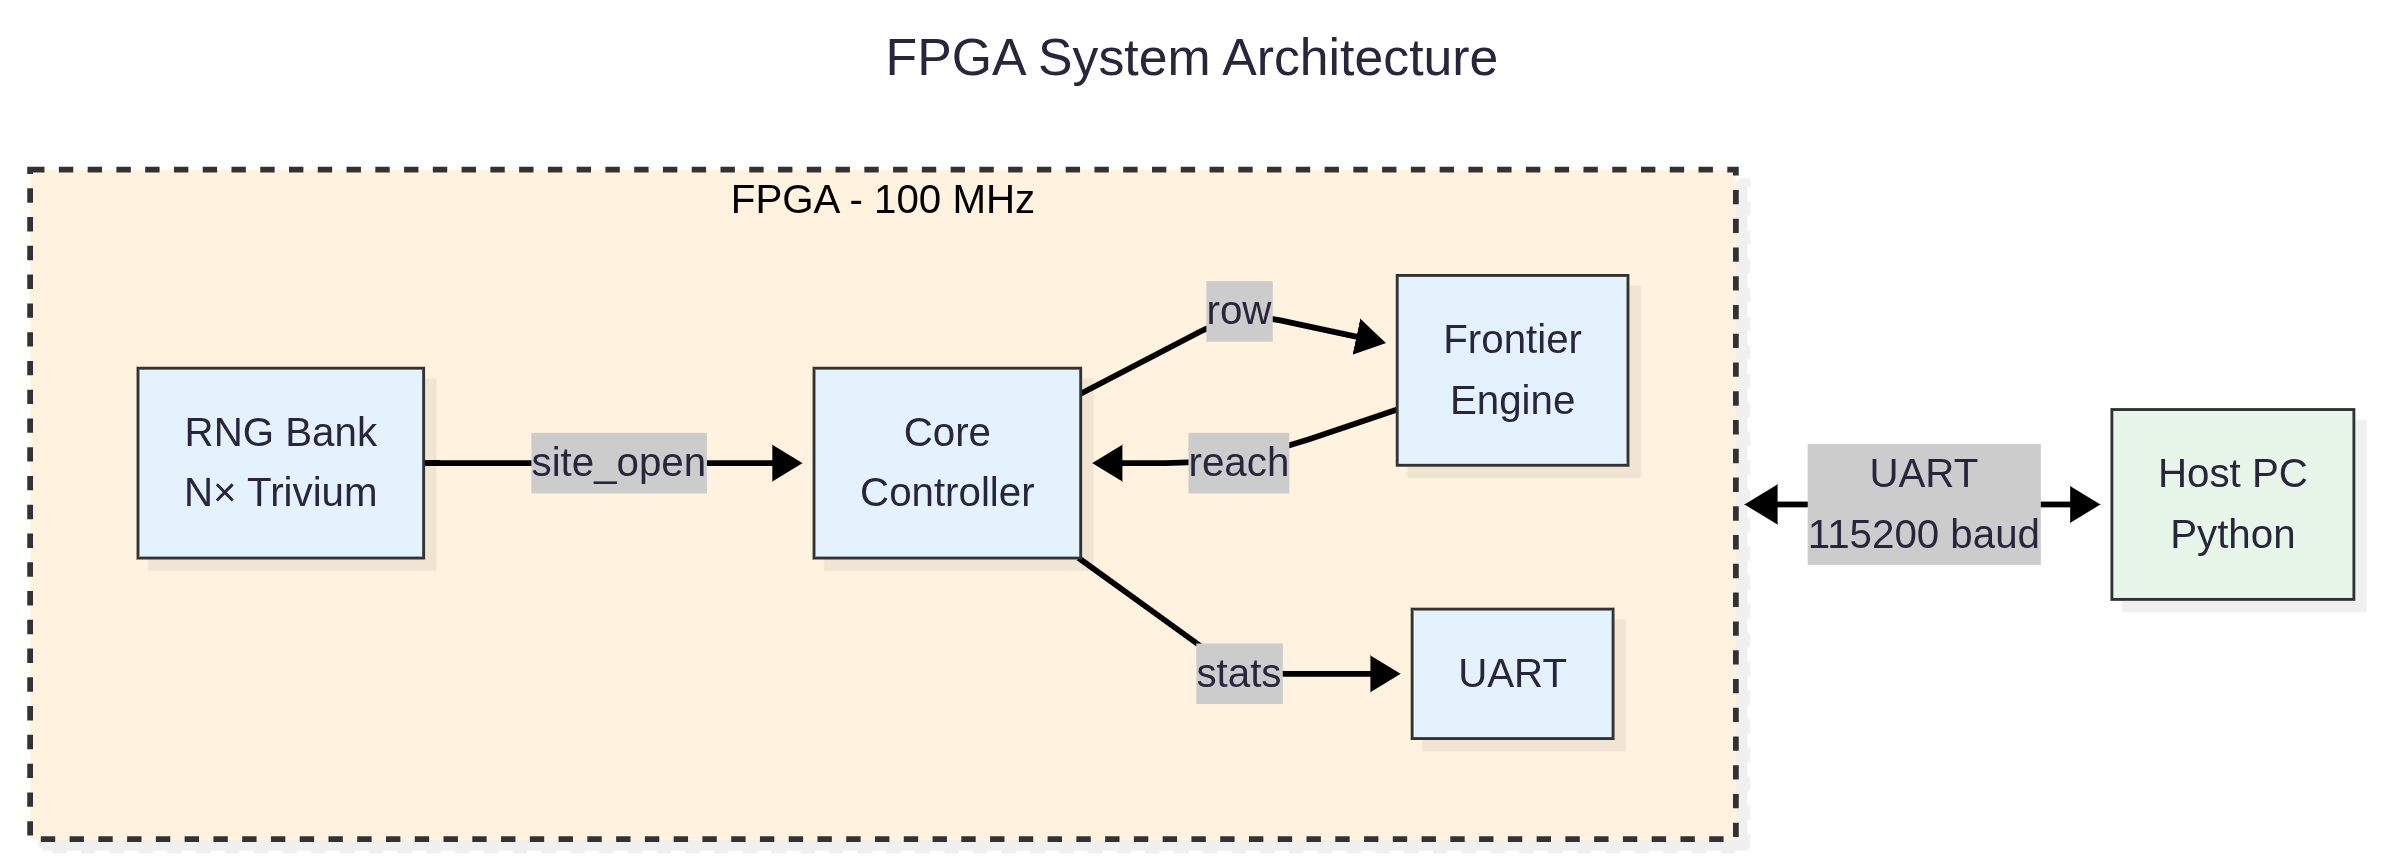
\includegraphics[width=\textwidth]{system_diagram.png}
\end{frame}


\begin{frame}{RNG Bank — Architecture}
  \begin{itemize}
    \item \alert{$N_{\text{rows}}$ independent} Trivium stream ciphers, one per grid column
    \item $N_{\text{rows}}$ is a \textbf{synthesis-time generic} (\texttt{N\_ROWS\_G}), default 64
    \item Synthesized for 64, 128, or 180 — same throughput, different resource usage
  \end{itemize}

  \vspace{0.1cm}
  \centering
  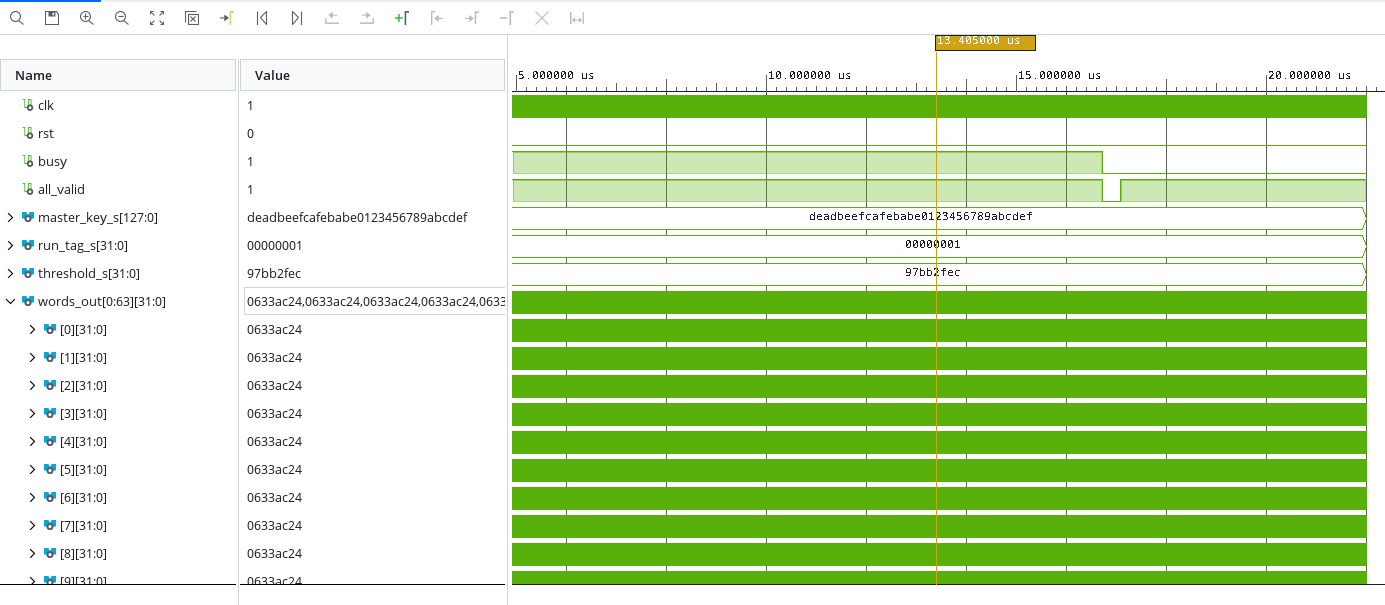
\includegraphics[width=0.85\textwidth]{sim_rng_warmup.png}

  \vspace{0.1cm}
  \textbf{AES-CTR seeding:} 128-bit key loaded, all 64 streams initialized in parallel
\end{frame}

\begin{frame}{RNG Bank — Seeding \& Output}
  \begin{columns}
    \column{0.68\textwidth}
    \textbf{AES-CTR Seeding:}
    \begin{itemize}
      \item For $N_{\text{rows}}=64$: 1536 cycles ($2N$ AES blocks $\times$ 12 cyc)
      \item Trivium warmup: 36 cycles (1152 bits $\div$ 32)
      \item \alert{Total: $\approx$1573 cycles} ($\approx$15.7 $\mu$s at 100 MHz)
    \end{itemize}
    \column{0.3\textwidth}
  \textbf{Per cycle output:}
  \begin{itemize}
    \item $N_{\text{rows}}$ random 32-bit words
  \end{itemize}
  \end{columns}

  \vspace{0.3cm}
    \centering
    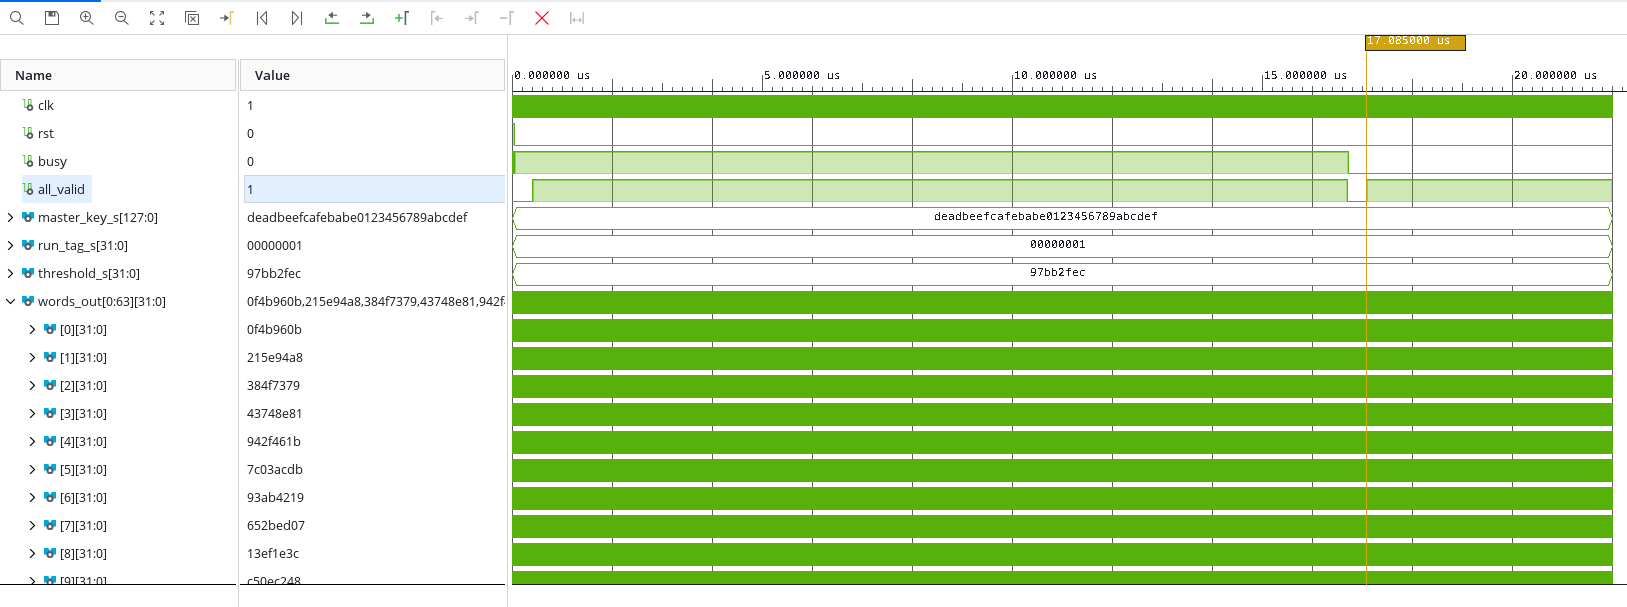
\includegraphics[width=.85\textwidth]{sim_rng_valid.png}

\end{frame}

\begin{frame}{Frontier Engine — Row-Wise Algorithm}
  \textbf{Problem:} determine if a top-to-bottom path exists without storing the full grid.

  \vspace{0.2cm}
  \textbf{Algorithm (per row):} $i$ is the \emph{horizontal} position within the row ($0 \le i < N_{\text{rows}}$).
  \begin{enumerate}
    \item \alert{Vertical seed:} $\text{seed}[i] = \text{open}[i] \land \text{prev\_reach}[i]$
    \item \alert{Horizontal closure (fixed point):} $\text{reach}[i] = \text{seed}[i] \lor (\text{open}[i] \land (\text{reach}[i{-}1] \lor \text{reach}[i{+}1]))$
  \end{enumerate}

  \vspace{0.3cm}
  \centering
  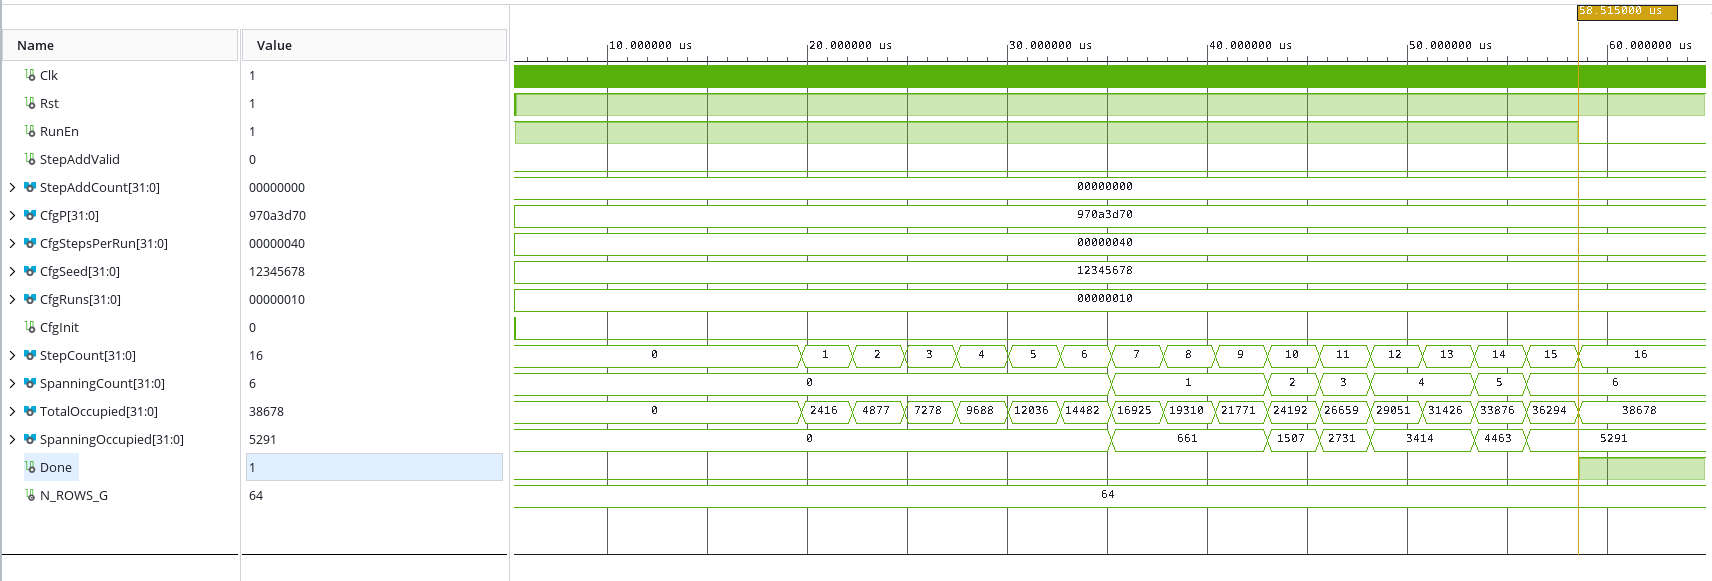
\includegraphics[width=0.7\textwidth]{sim_core.png}

  \vspace{0.2cm}
  \textbf{Bidirectional prefix scan:} resolves in $\log_2 N_{\text{rows}}$ stages (6 for $N=64$) in a single cycle
\end{frame}

\begin{frame}{Frontier Engine — VHDL Pipeline}

    \textbf{3-stage pipeline:}
    \begin{itemize}
      \item RUN\_READY $\to$ RUN\_COMPUTE $\to$ RUN\_SAVE
      \item \alert{3 cycles/row} core computation
      \item \alert{4 cycles/row end-to-end} (includes registered handshake)
      \item Only 2 rows of state buffered
    \end{itemize}

    \centering
    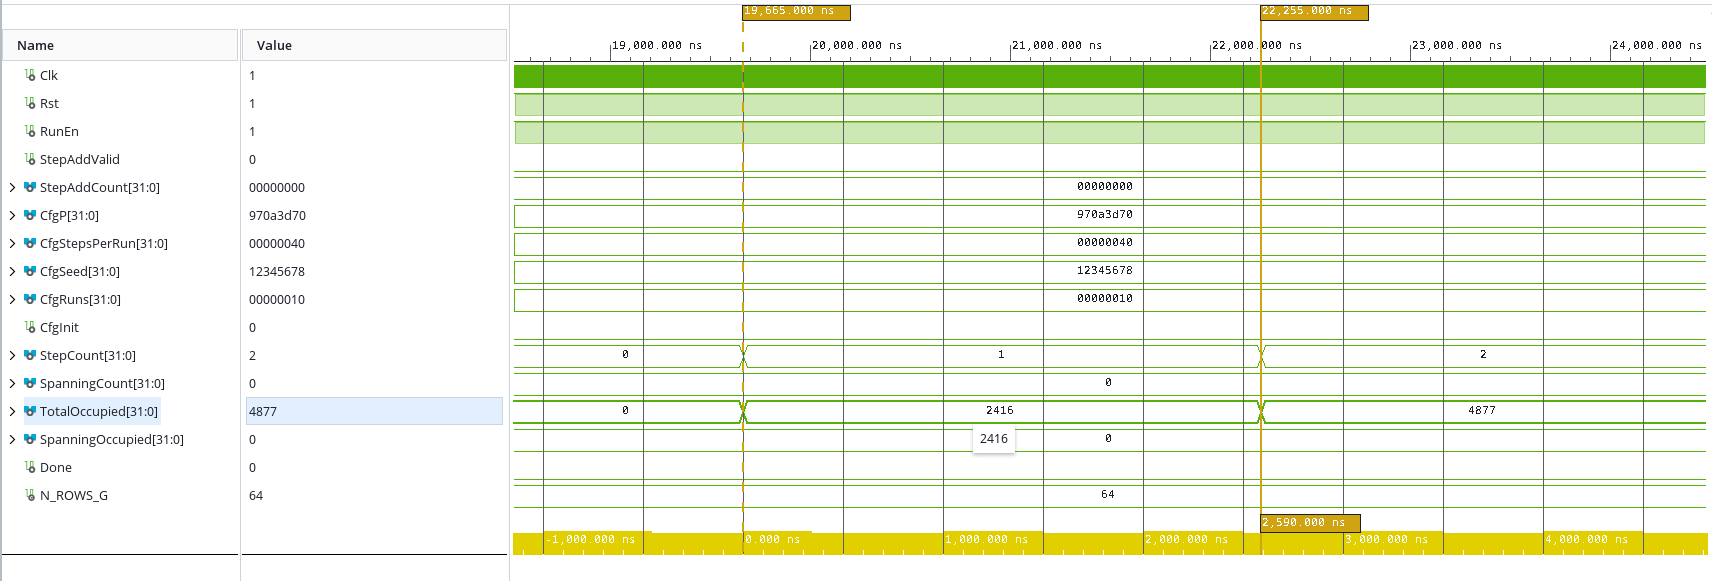
\includegraphics[width=0.85\textwidth]{sim_core_single.png}


  \vspace{0.3cm}
  \textbf{Validation:} 1000 random tests, exact match with BFS reference
\end{frame}

\begin{frame}{Core Controller — State Machine}
  \centering
  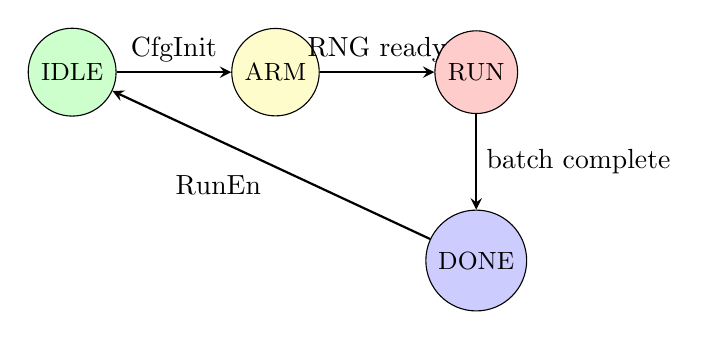
\begin{tikzpicture}[
    state/.style={circle, draw, minimum size=0.08\textwidth, align=center, font=\small},
    arrow/.style={->, thick, >=stealth}
  ]
    \node[state, fill=green!20] (idle) {IDLE};
    \node[state, right=0.12\textwidth of idle, fill=yellow!20] (arm) {ARM};
    \node[state, right=0.12\textwidth of arm, fill=red!20] (run) {RUN};
    \node[state, below=0.1\textwidth of run, fill=blue!20] (done) {DONE};

    \draw[arrow] (idle) -- node[above] {CfgInit} (arm);
    \draw[arrow] (arm) -- node[above] {RNG ready} (run);
    \draw[arrow] (run) -- node[right] {batch complete} (done);
    \draw[arrow] (done) -- node[below left] {RunEn} (idle);
  \end{tikzpicture}

  \vspace{0.3cm}
  \textbf{Batch processing:}
  \begin{itemize}
    \item \texttt{CfgRuns} runs executed autonomously — no host intervention
    \item Accumulators (32-bit): StepCount, SpanningCount, TotalOccupied, SpanningOccupied
    \item RNG runs continuously — no cycle wasted waiting for random numbers
  \end{itemize}
\end{frame}

\begin{frame}{UART Protocol — 16-Byte Frames}
  \begin{columns}[t]
    \column{0.6\textwidth}
    \textbf{Request (host $\to$ FPGA):}
    {\footnotesize
    \begin{tabular}{lll}
      \toprule
      Word & Field & Purpose \\
      \midrule
      0 & CfgP (UQ32) & Probability $p$ \\
      1 & CfgSeed & RNG seed \\
      2 & CfgStepsPerRun & Grid height \\
      3 & CfgRuns & Batch size \\
      \bottomrule
    \end{tabular}
    }

    \vspace{0.2cm}
    \textbf{Response (FPGA $\to$ host):}
    {\footnotesize
    \begin{tabular}{lll}
      \toprule
      Word & Field & Purpose \\
      \midrule
      0 & StepCount & Runs completed \\
      1 & SpanningCount & Spanning runs \\
      2 & TotalOccupied & Total occupied site\\
      3 & SpanningOccupied & Reachable sites \\
      \bottomrule
    \end{tabular}
    }

    \column{0.4\textwidth}
    \textbf{Details:}
    \begin{itemize}
      \item 115200 baud
      \item Wire time: $\approx$2.78 ms
      \item Linux termios raw mode
      \item Fixed-point: $p = \text{CfgP} / 2^{32}$
    \end{itemize}
  \end{columns}
\end{frame}

\begin{frame}{UART Protocol — End-to-End Simulation}
  \centering
  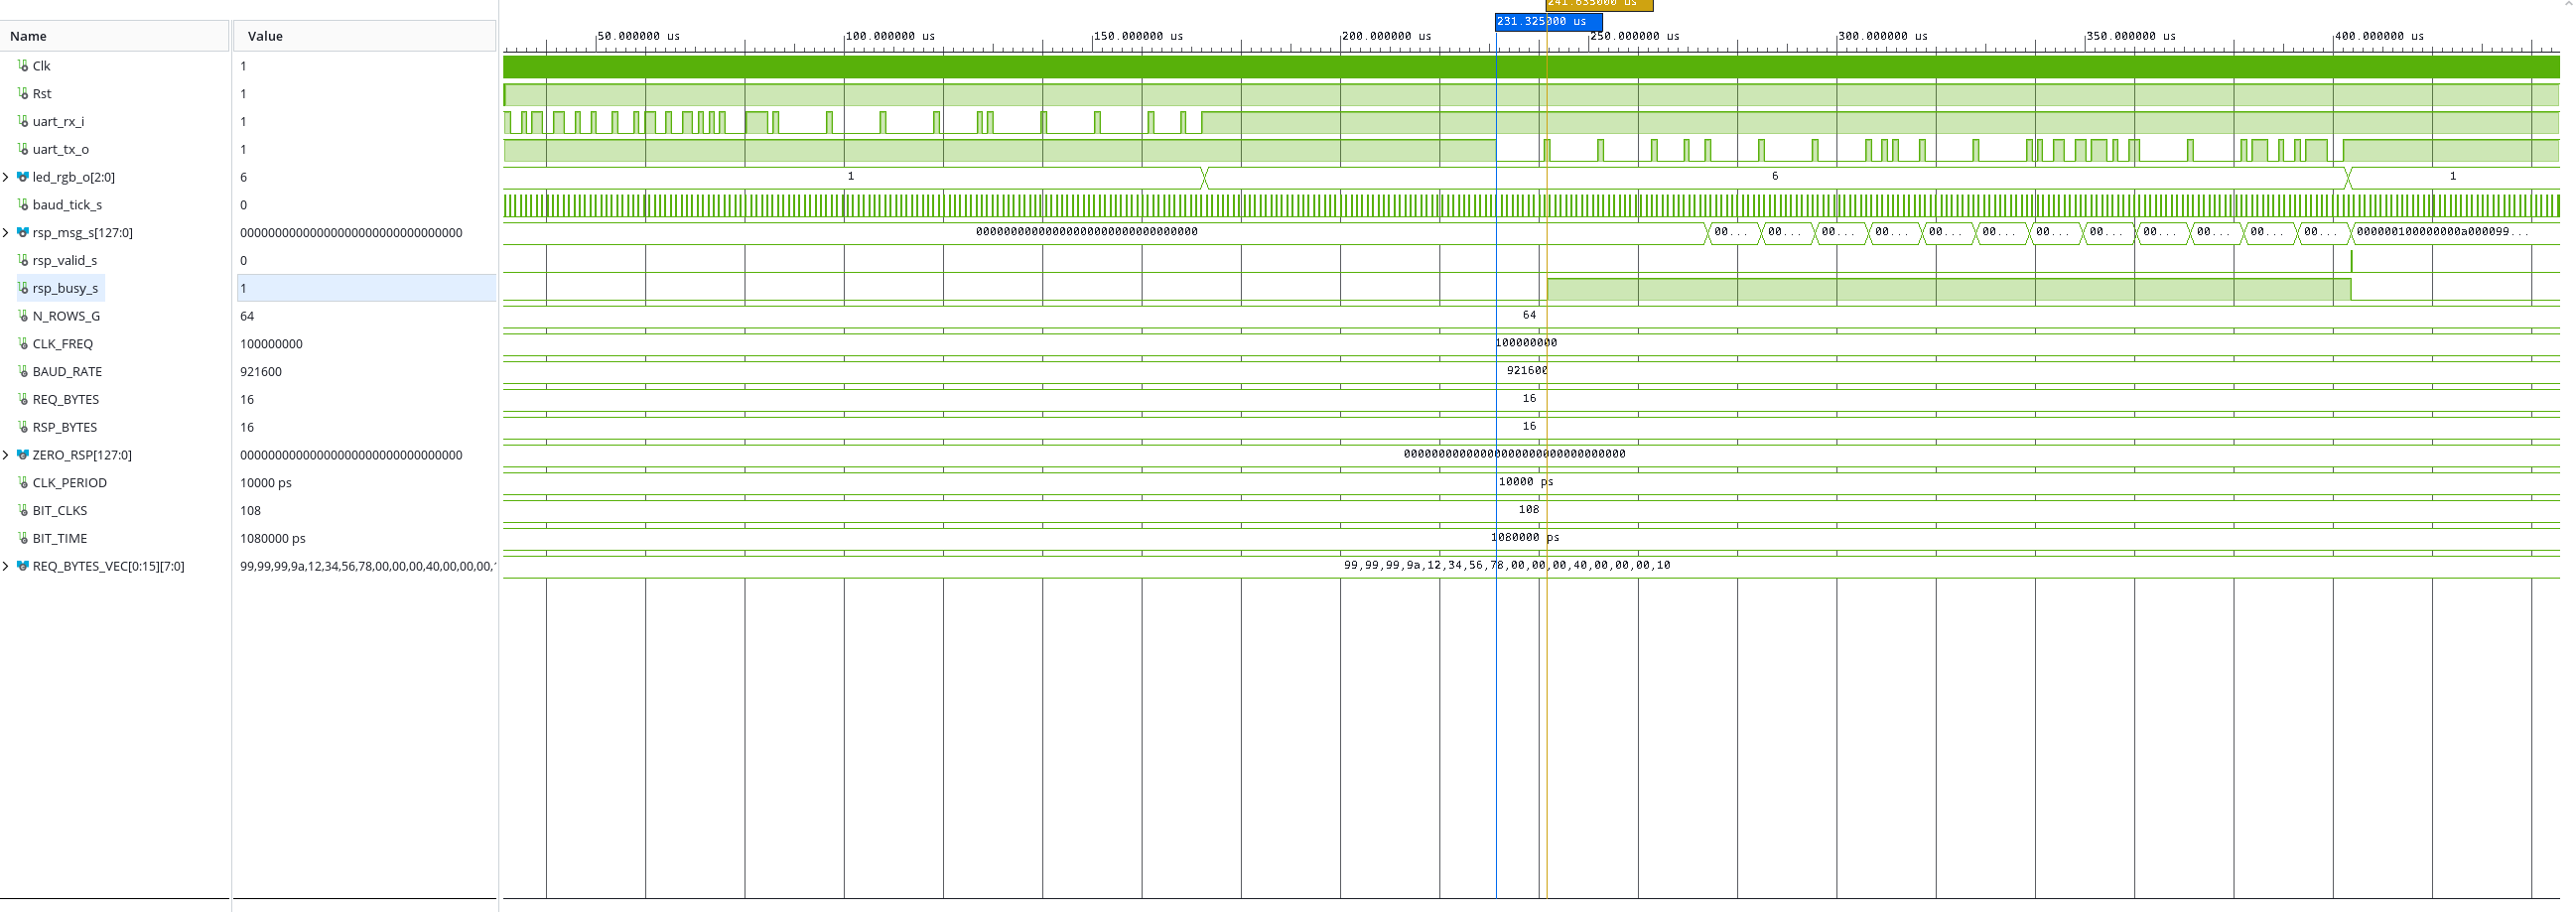
\includegraphics[width=\textwidth]{sim_uart_top.png}
\end{frame}


% ============================================================
%  SECTION 3 — Validation
% ============================================================
\section[Val.]{Validation}

\begin{frame}{Three-Way Comparison — Full Range}
  \centering
\begin{columns}
\column{0.3\textwidth}
  \begin{itemize}
    \item BFS (undirected) vs SW FPGA (directed) vs HW FPGA
    \item 20 points, 1000 runs each
    \item Directed percolation threshold is \alert{higher} ($\pc \approx 0.605$) than isotropic ($\pc \approx 0.593$)
  \end{itemize}
  \column{0.7\textwidth}
  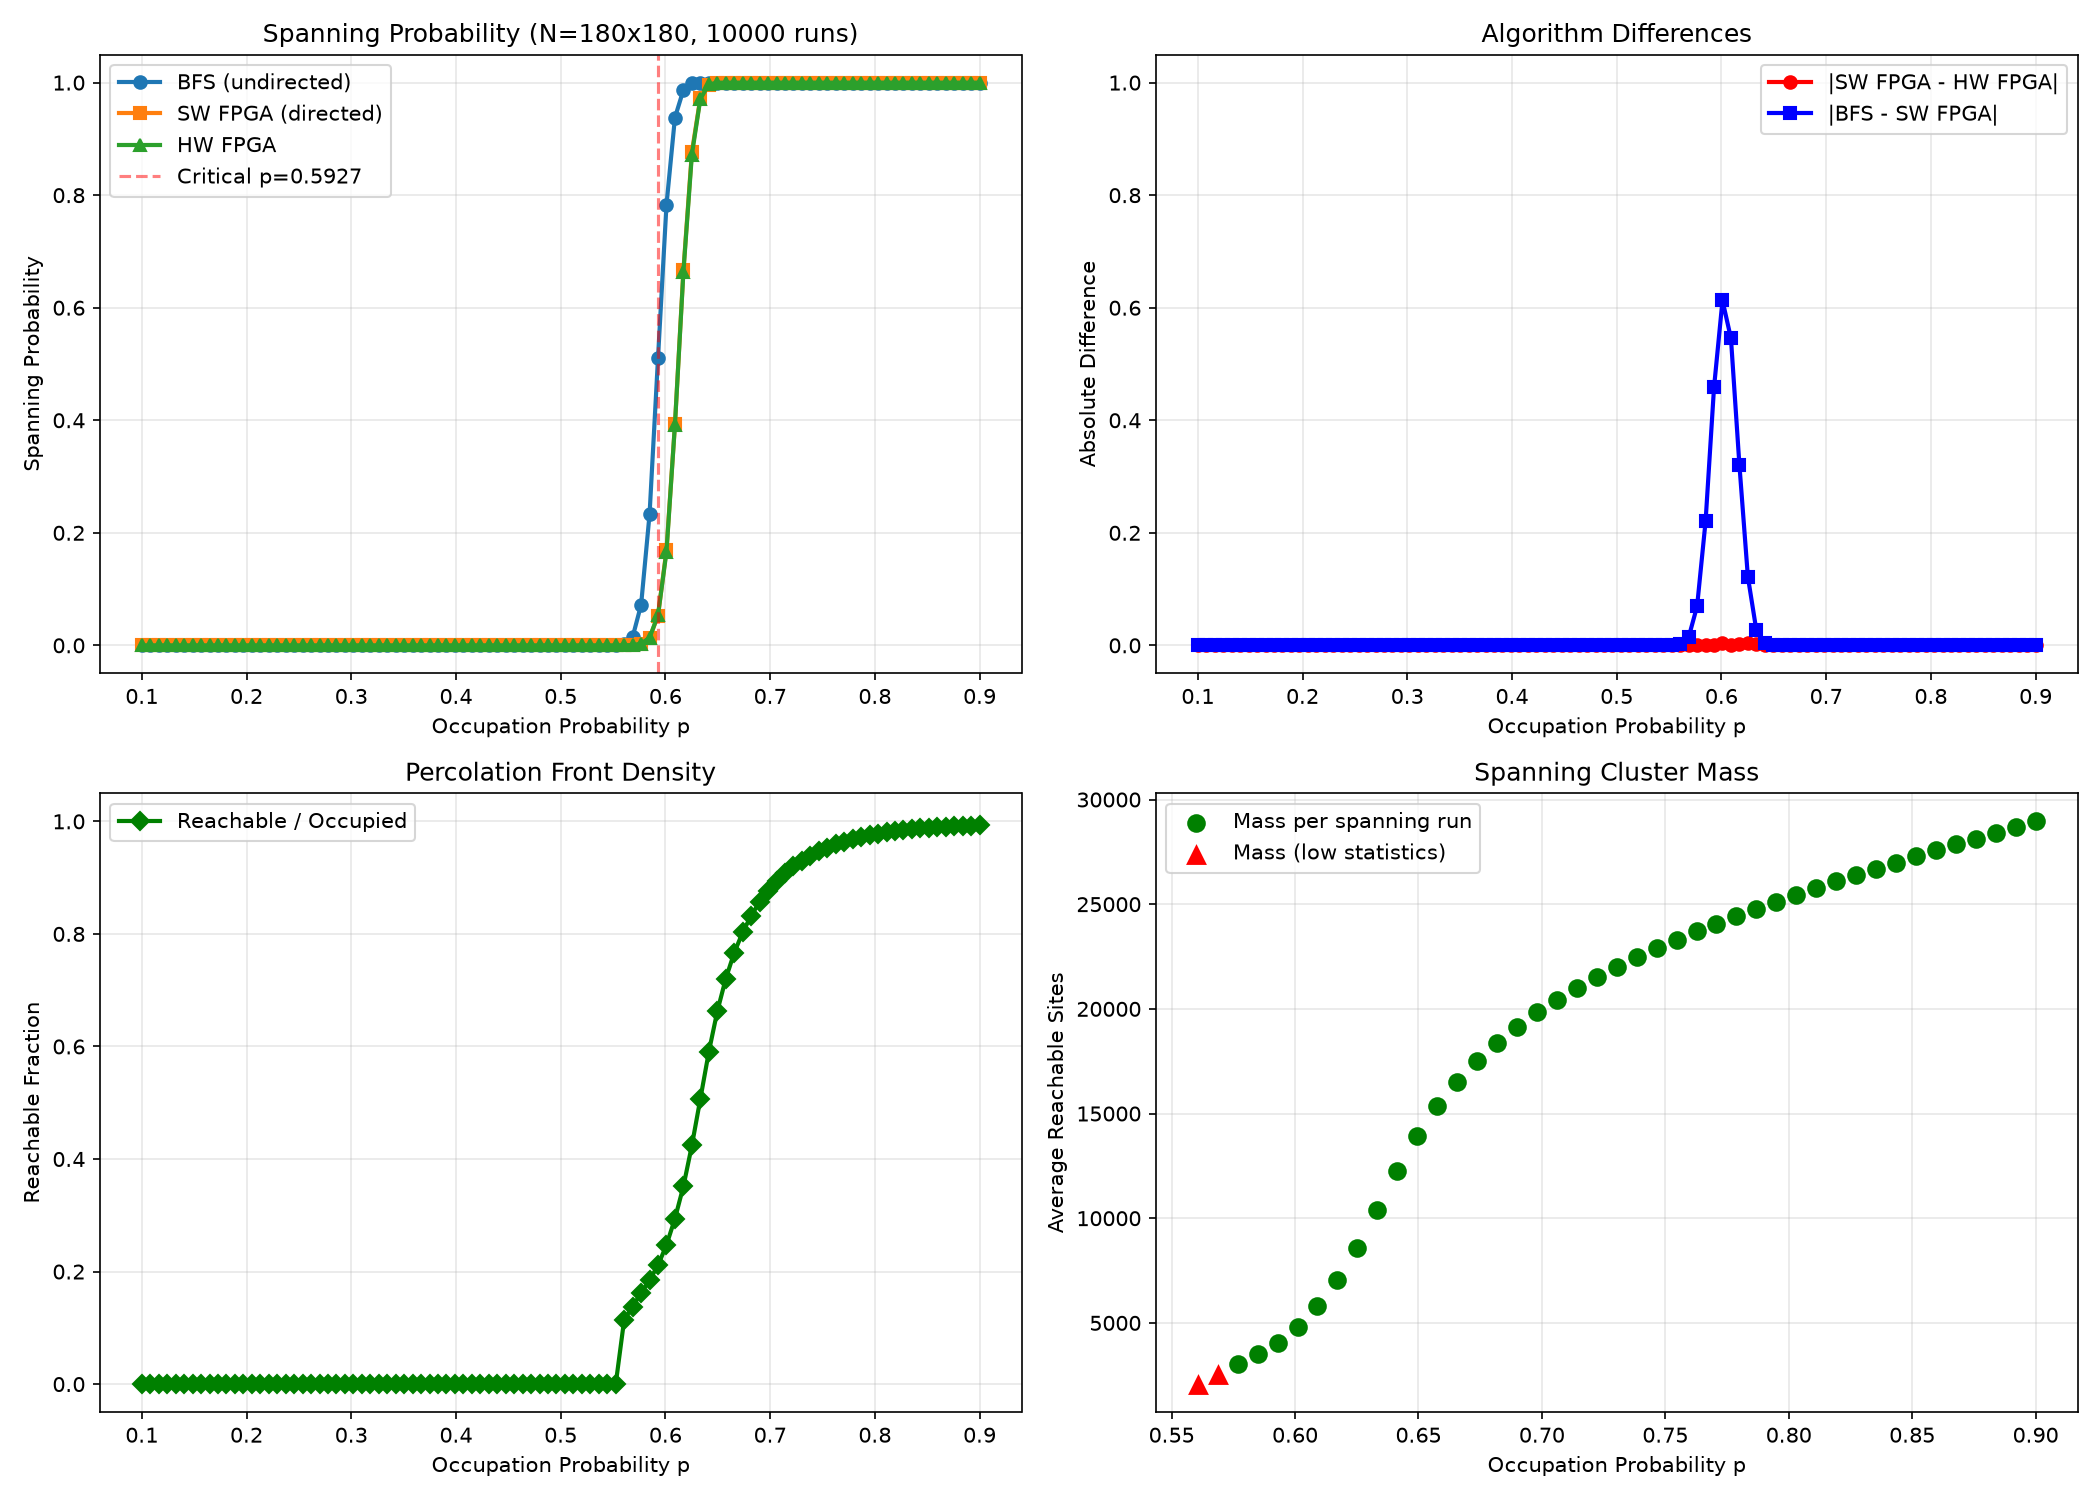
\includegraphics[width=\textwidth]{three_way_comparison.png}
\end{columns}
\end{frame}

\begin{frame}{Three-Way Comparison — Threshold Region}
  \centering
\begin{columns}
\column{0.3\textwidth}
  \begin{itemize}
    \item Zoom around the critical region
    \item 100 points, 1000 runs each
    \item Perfect agreement between software model and hardware implementation
  \end{itemize}
  \column{0.7\textwidth}
  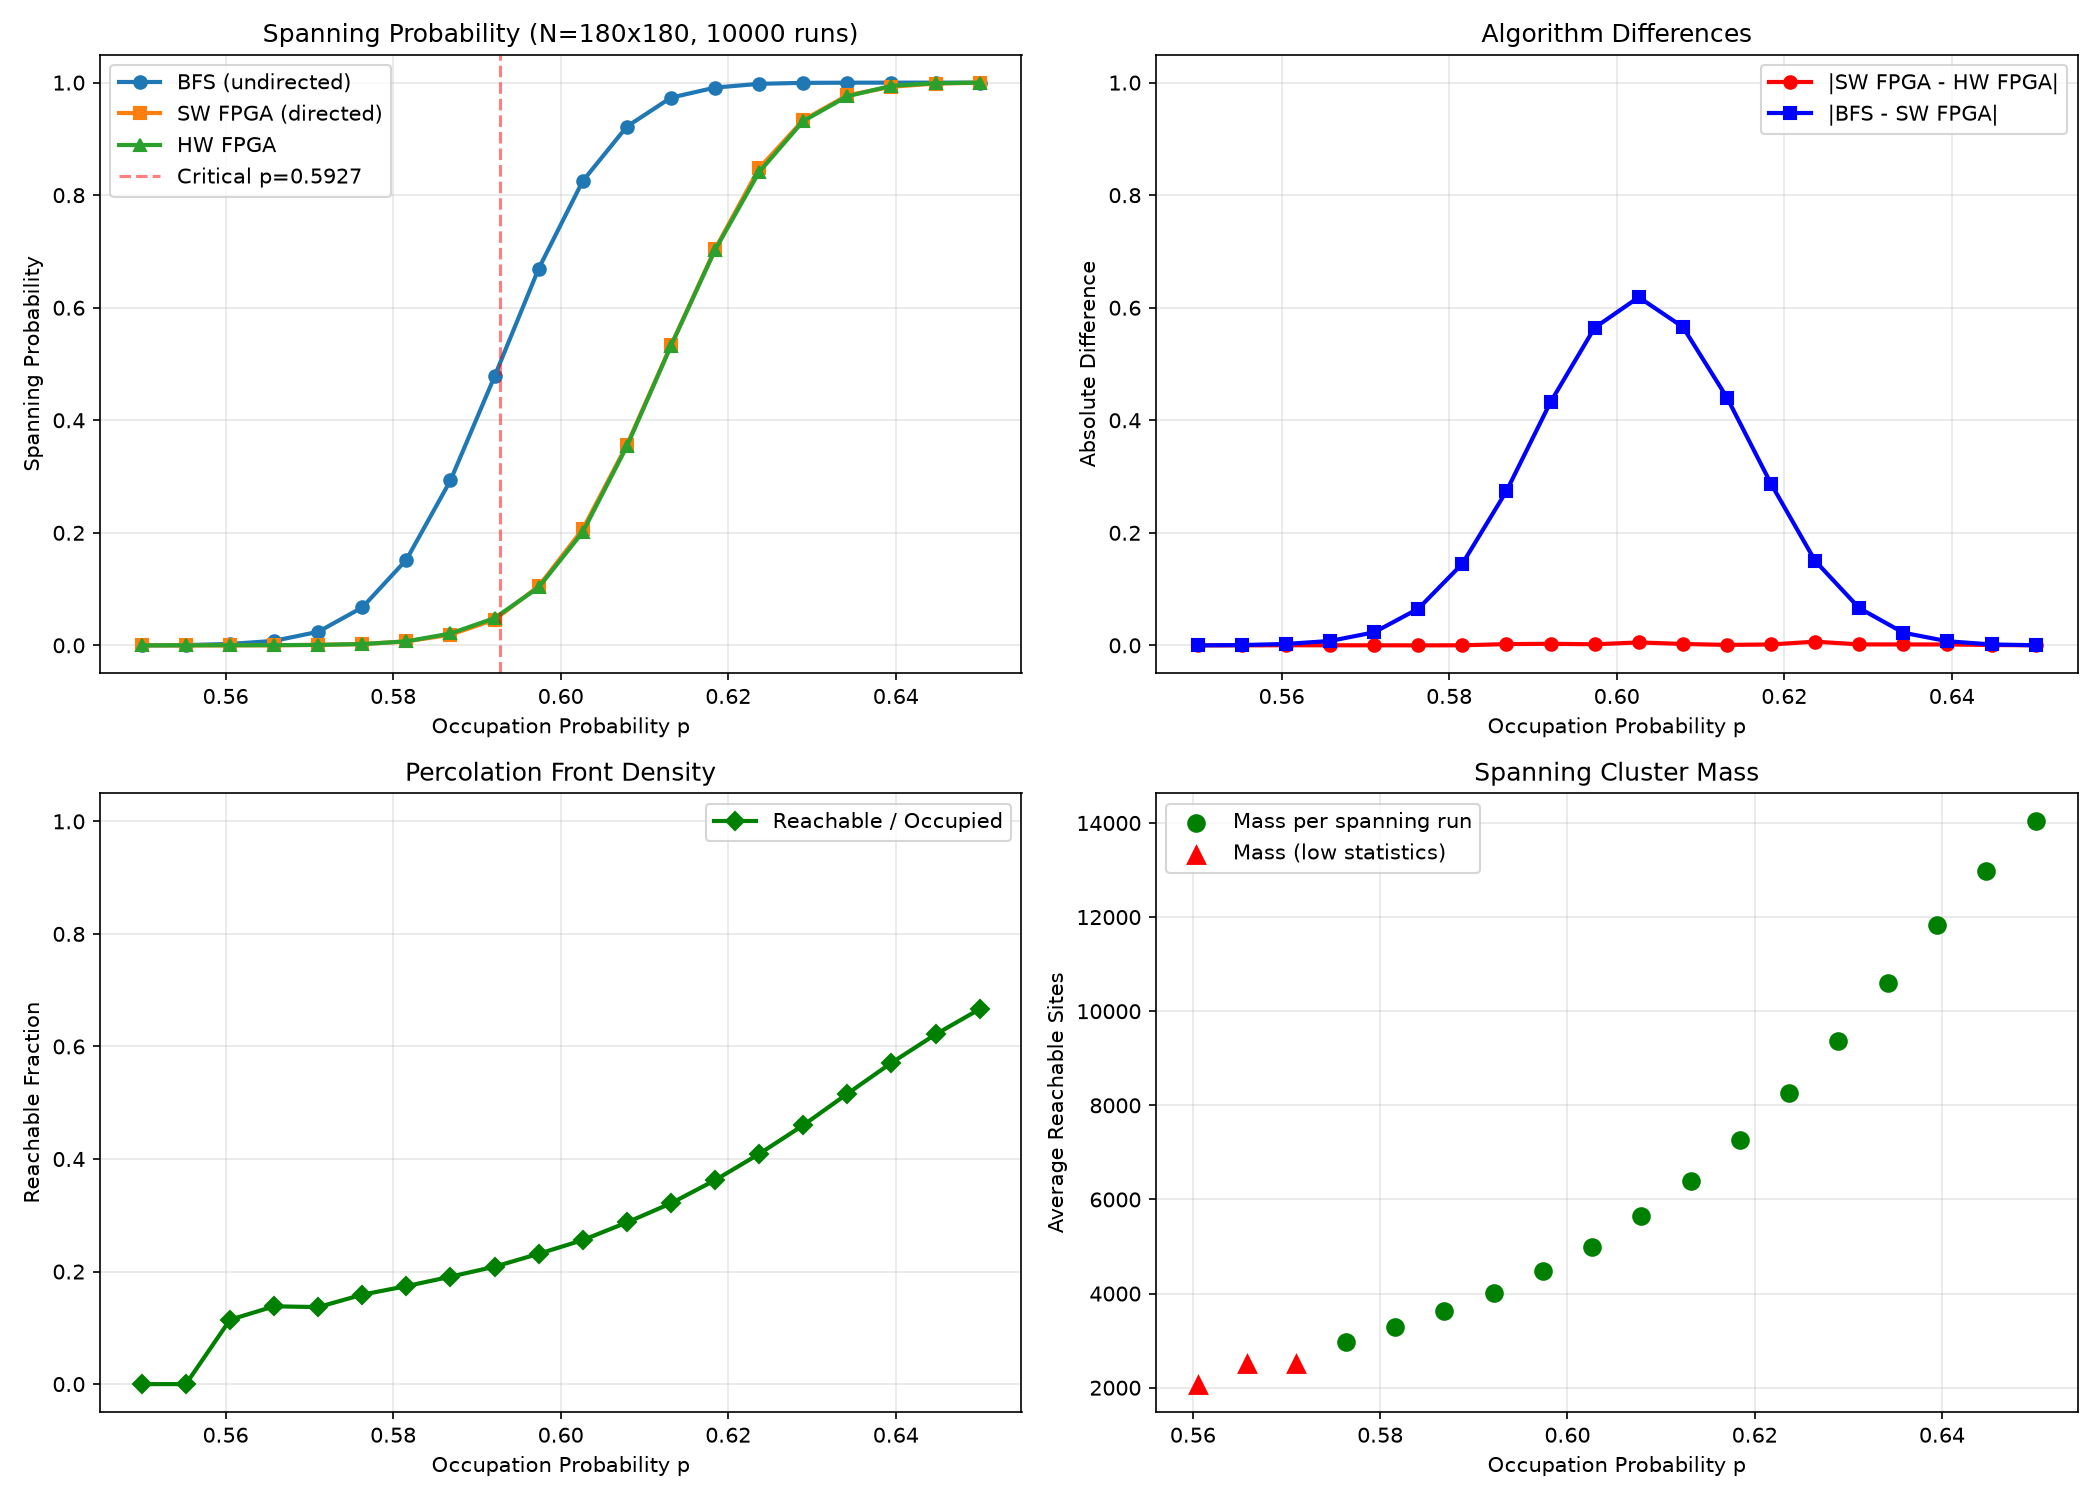
\includegraphics[width=\textwidth]{three_way_comparison_zoom.png}
\end{columns}
\end{frame}

\begin{frame}{Occupancy Bias — RNG Accuracy}
  \centering
  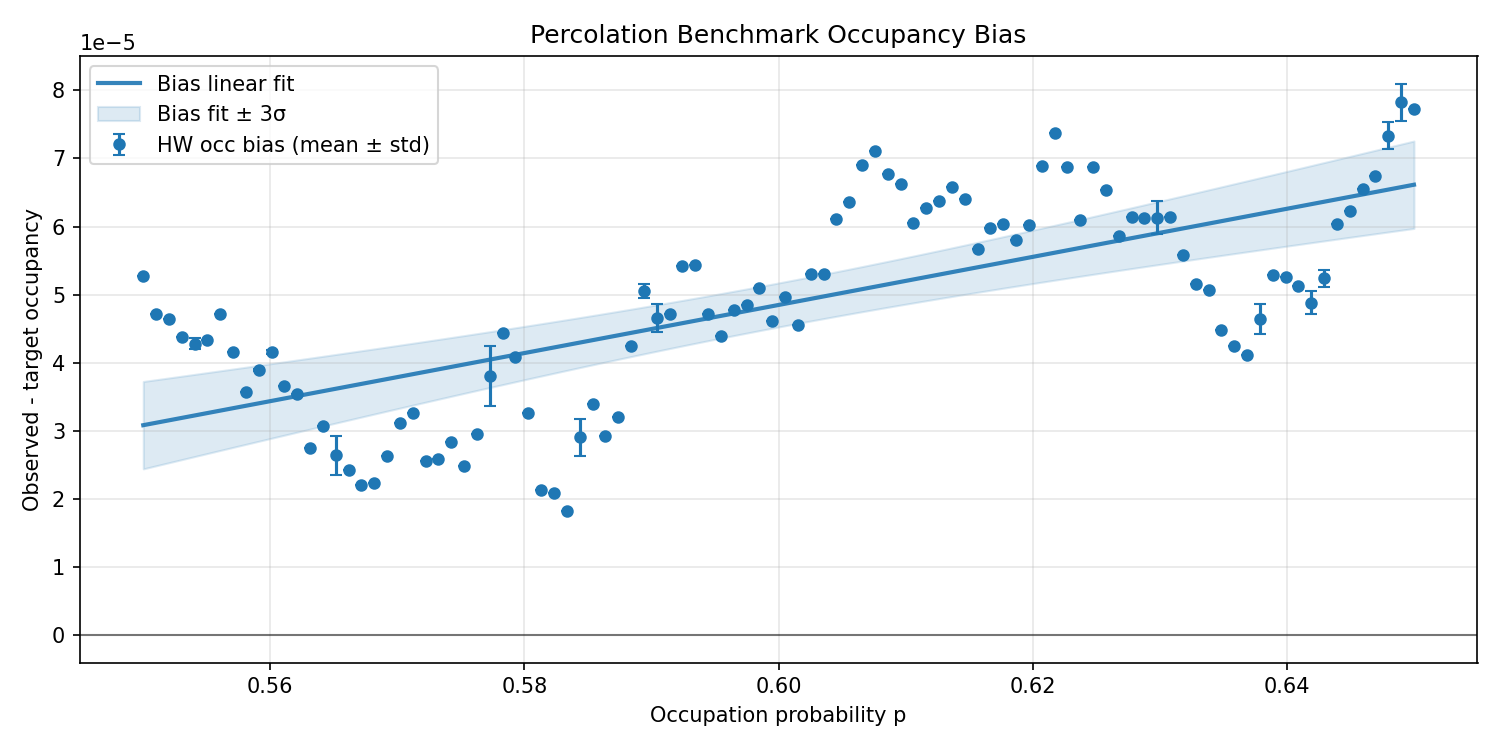
\includegraphics[width=0.65\textwidth]{occupancy_bias.png}
  \vspace{0.2cm}
  \begin{itemize}
    \item Bias $= \langle p_{\text{measured}} \rangle - p_{\text{target}}$
    \item \alert{Maximum bias $< 0.001$} across full $p$ range
    \item No systematic trend — RNG is unbiased
  \end{itemize}
\end{frame}

% ============================================================
%  SECTION 4 — FPGA Engineering Results
% ============================================================
\section{FPGA Engineering Results}

%% \begin{frame}{Latency vs Batch Size — Amdahl Speedup}
%%   \centering
%%   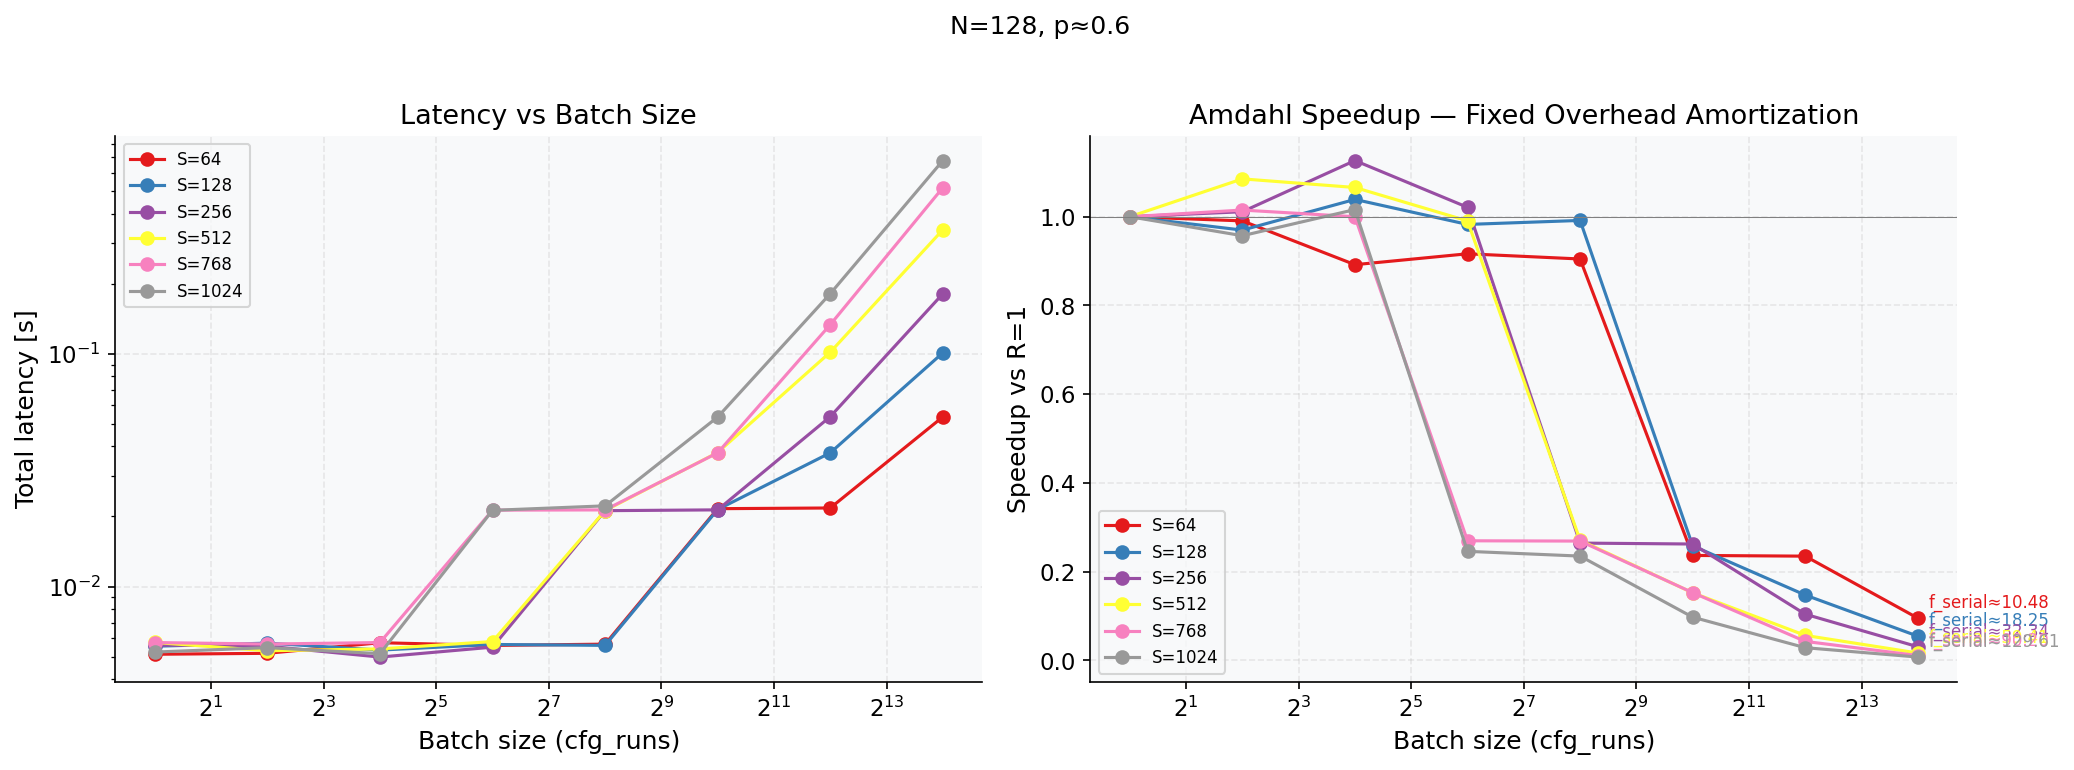
\includegraphics[width=0.45\textwidth]{latency_vs_batch.png}
%%   \vspace{0.2cm}
%%   \begin{itemize}
%%     \item Fixed UART overhead $\approx$2.78 ms dominates at small $R$
%%     \item Speedup follows Amdahl's law: serial fraction $f_{\text{serial}} \approx 0.2$--$0.4$
%%     \item Break-even batch size: $R \approx 100$--$1000$ depending on grid height
%%   \end{itemize}
%% \end{frame}

\begin{frame}{Asymptotic Throughput — Amdahl Decomposition}
  \centering
  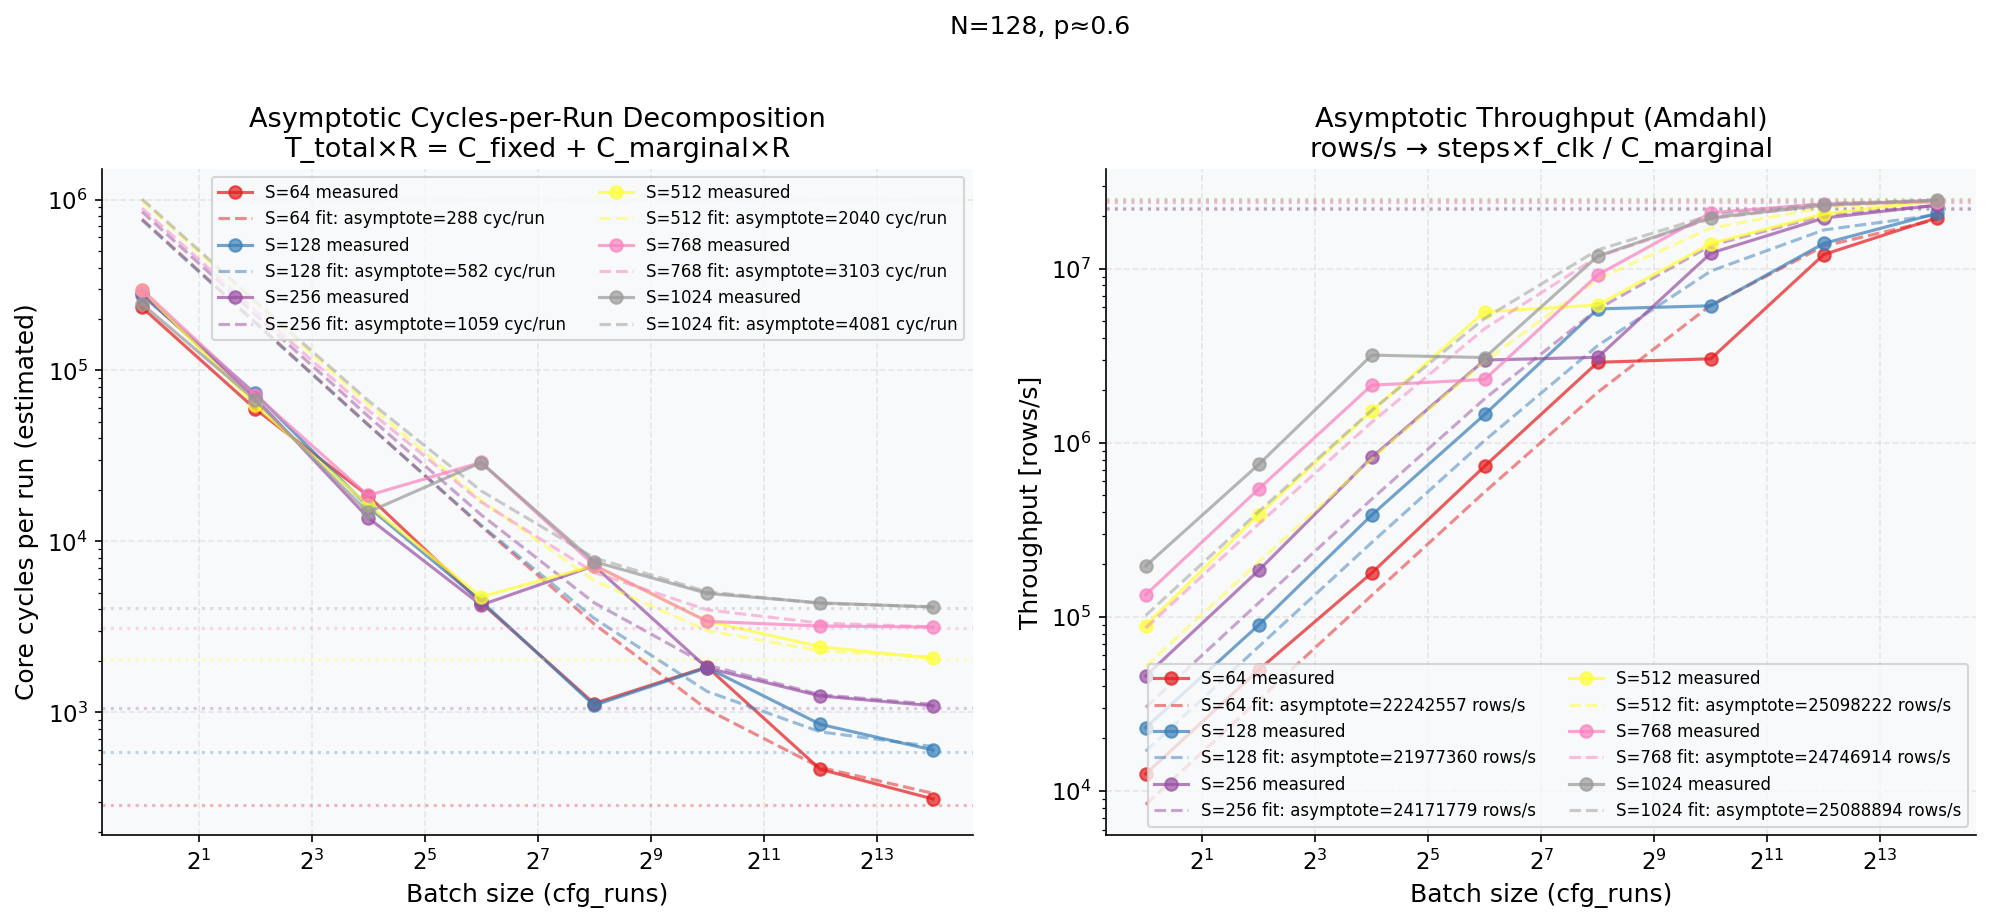
\includegraphics[width=\textwidth]{breakdown_throughput.png}
\end{frame}

\begin{frame}{Theoretical vs practical efficiency}
  \centering
  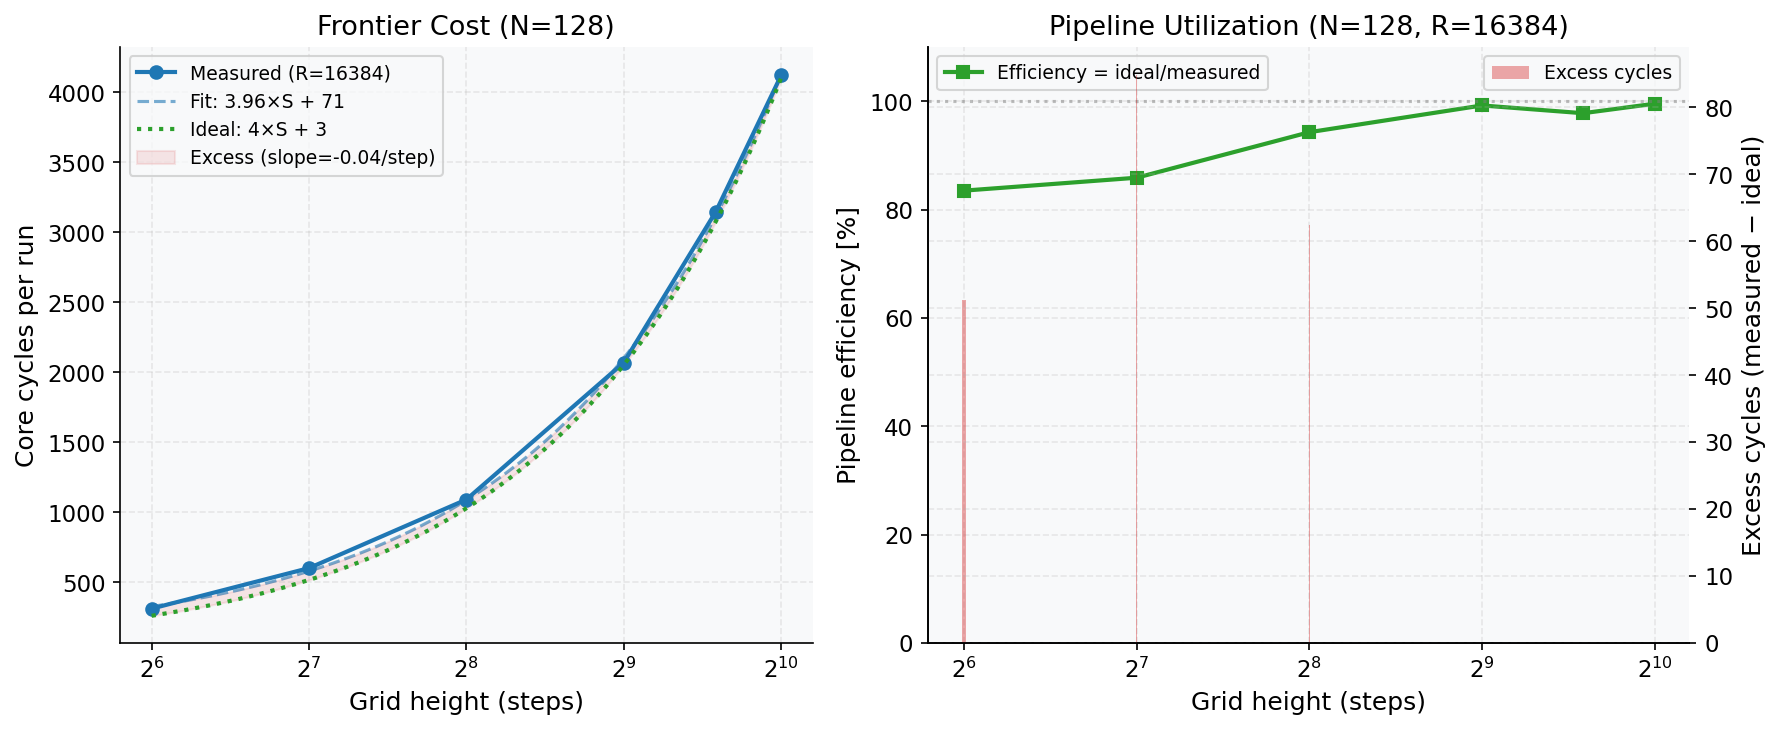
\includegraphics[width=\textwidth]{pipeline_efficiency.png}
\end{frame}

\begin{frame}{Model and Speed results}
  \textbf{Model:} $T_{\text{total}} \times R = C_{\text{fixed}} + C_{\text{marginal}} \times R$

  \vspace{0.2cm}
  \begin{itemize}
    \item $C_{\text{fixed}}$: UART + host overhead (one-time per request)
    \item $C_{\text{marginal}}$: per-run core cost (asymptote at large $R$)
    \item \textbf{Throughput:} $\displaystyle \frac{\text{rows}}{\text{s}} = \frac{\text{steps} \times f_{\text{clk}}}{C_{\text{marginal}}}$
\end{itemize}
  \textbf{Results:}
  \begin{itemize}
    \item Asymptote matches theoretical $4 \times S$ cycles/run (3 frontier + 1 handshake)
    \item Measured: $C_{\text{core}} = 3.96 \times S + \text{const}$ (vs ideal $4 \times S$)
    \item For $N=64$: measured asymptote $\approx 288$ cycles/run vs theoretical $4N+3 = 259$ ($\approx$11\% state-machine overhead at the latest point we measured)
    \item \alert{Efficiency: $\approx$100\%} of achievable $4 \times S$ model
    \item Throughput scales with batch size, saturating at $\sim 2.5 \times 10^7$ rows/s
  \end{itemize}
\end{frame}




% ============================================================
%  SECTION 5 — Physics Results
% ============================================================
\section{Physics Results}

\begin{frame}{Finite-Size Scaling — Collapse}
  \centering
  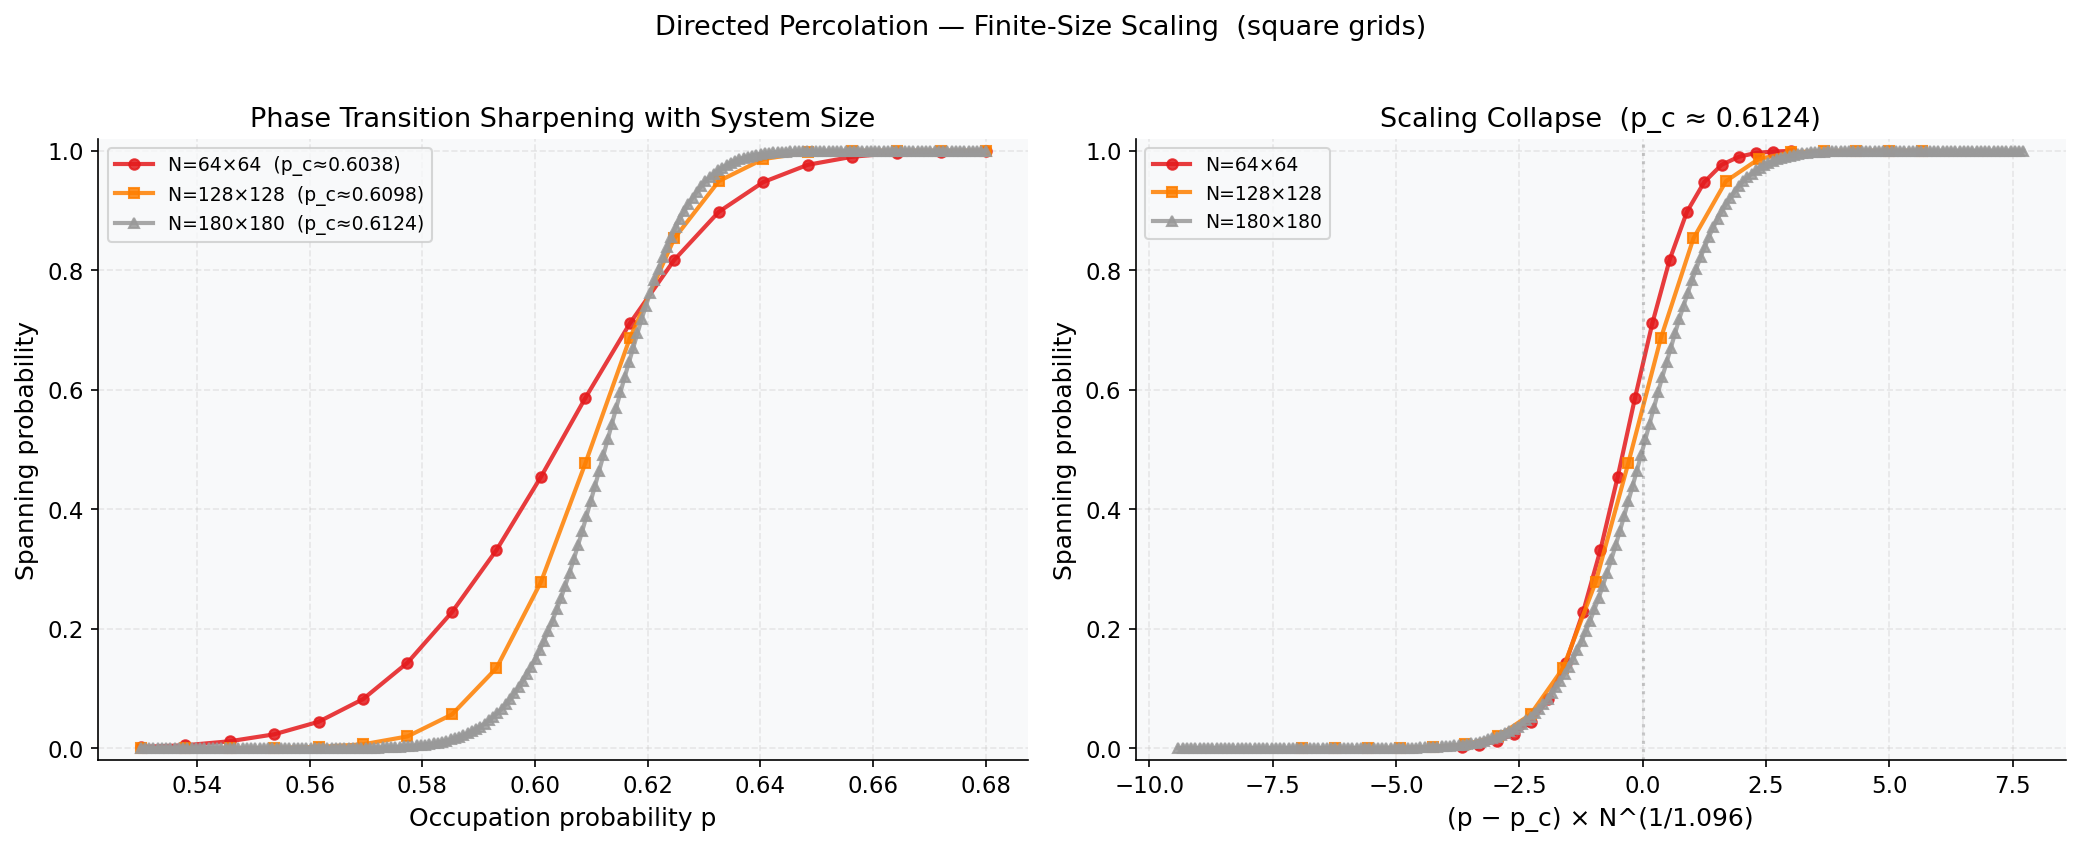
\includegraphics[width=0.75\textwidth]{finite_size_scaling.png}
  \vspace{0.2cm}
  \begin{itemize}
    \item Square grids: $N = 64, 128, 180$
    \item \alert{Perfect collapse} using DP exponent $\nu_{\|} = 1.096$
    \item Confirms the system belongs to the directed percolation universality class
  \end{itemize}
\end{frame}

\begin{frame}{Threshold Estimation — Bootstrap}
  \centering
  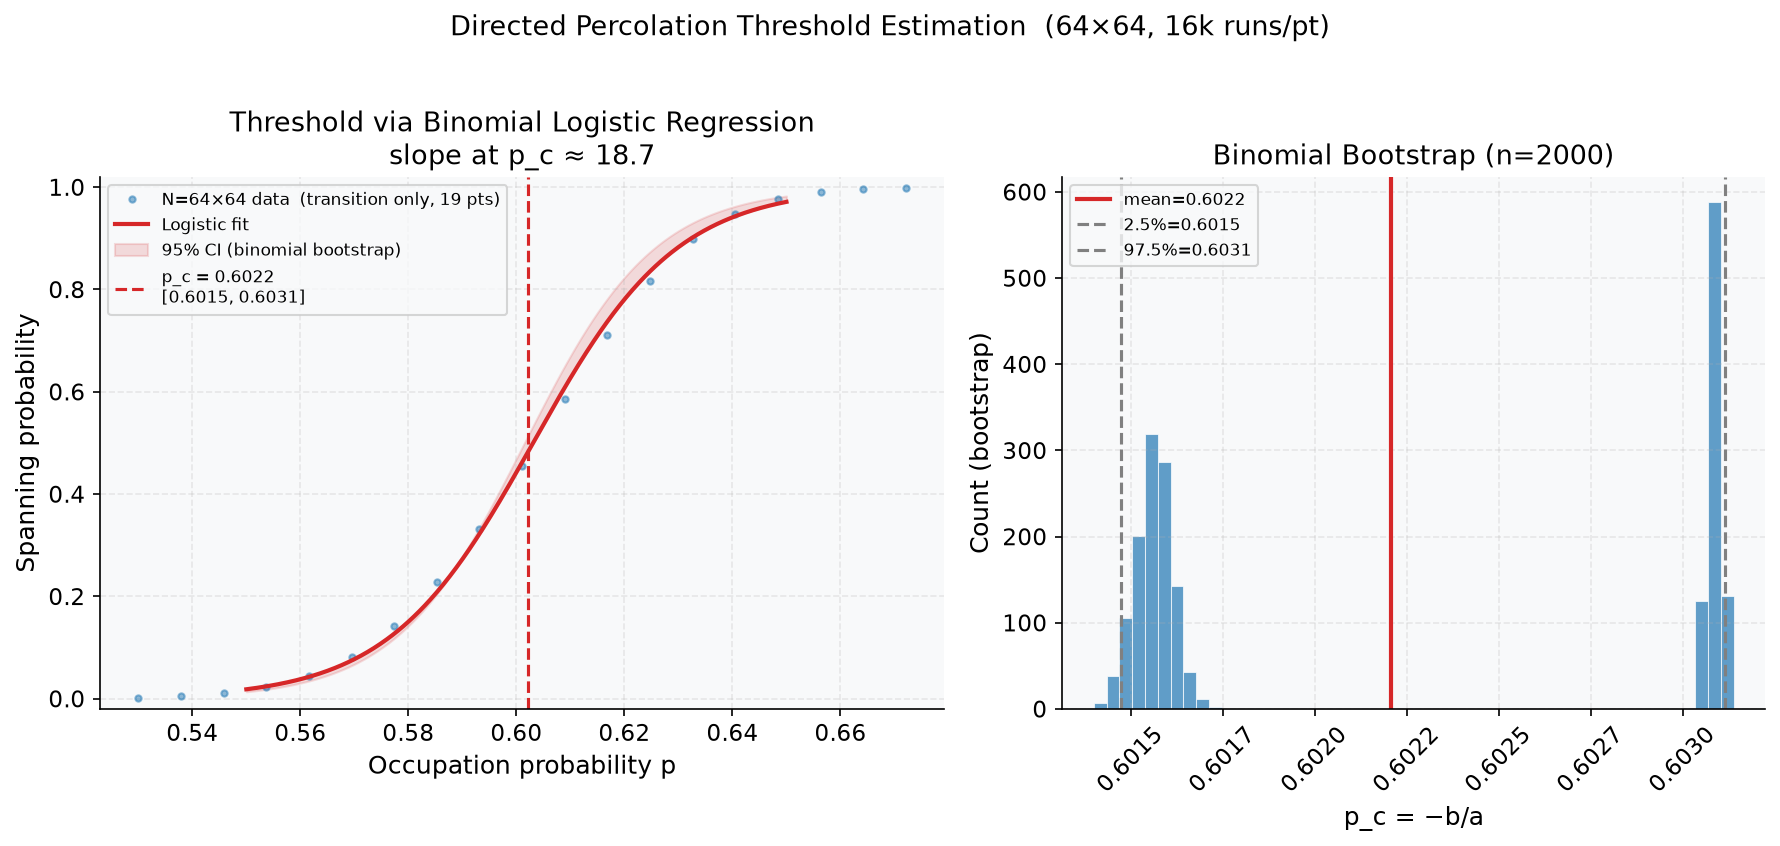
\includegraphics[width=0.55\textwidth]{threshold_bootstrap_64.png}\\

  \textbf{Method:} binomial logistic regression + 2000 bootstrap resamples
  \[
  P_{\text{span}}(p) = \frac{1}{1 + e^{-a(p - \pc)}}
  \]
  \begin{itemize}
    \item \alert{$\pc = 0.6022 \pm 0.0007$} (95\% CI)
    \item Fairly consistent with literature value $\approx 0.605$ for DP on $64\times64$
  \end{itemize}
\end{frame}

% ============================================================
%  SECTION 6 — Conclusions
% ============================================================
\section{Conclusions}



\begin{frame}{Thank You}
  \centering
  \vfill
  {\Huge Questions?}
  \vfill

  \textbf{Repository:} \url{https://github.com/tusca99/FPGA-project}

  \vspace{0.3cm}
  \small
  \begin{itemize}
    \item VHDL: percolation core, RNG bank, frontier engine
    \item Python: validation, benchmark, analysis
    \item Full documentation in \texttt{project/percolation\_core/}
  \end{itemize}
\end{frame}

\section{Backup}
\begin{frame}{Summary of Results}
  \begin{table}
    \centering
\resizebox{\textwidth}{!}{
    \begin{tabular}{lcc}
      \toprule
      \textbf{Metric} & \textbf{Value} & \textbf{Notes} \\
      \midrule
      Clock frequency & 100 MHz & Single-clock, Artix-7 \\
      Grid width $N_{\text{rows}}$ & 64 (128, 180) & Compile-time generic \\
      Frontier pipeline & 3 cycles/row & READY $\to$ COMPUTE $\to$ SAVE \\
      Cycles per run ($N{\times}N$) & $4N + 3$ & e.g. $N=64 \to \approx 259$ \\
      Pipeline efficiency & $\approx$100\% & Of achievable $4\times S$ model \\
      Throughput & $\sim 10^9$ cells/s & At 100 MHz ($\sim$2.5$\times$10$^7$ rows/s $\times$ 64) \\
      Occupancy bias & $< 0.001$ & RNG accuracy \\
      Critical threshold $\pc$ & $0.6047 \pm 0.0002$ & DP universality class \\
      UART overhead & $\approx$2.78 ms & 115200 baud, 32 bytes \\
      \bottomrule
    \end{tabular}
}
  \end{table}
\end{frame}

\begin{frame}{Grid-Height Invariance \& Determinism}
    \centering
    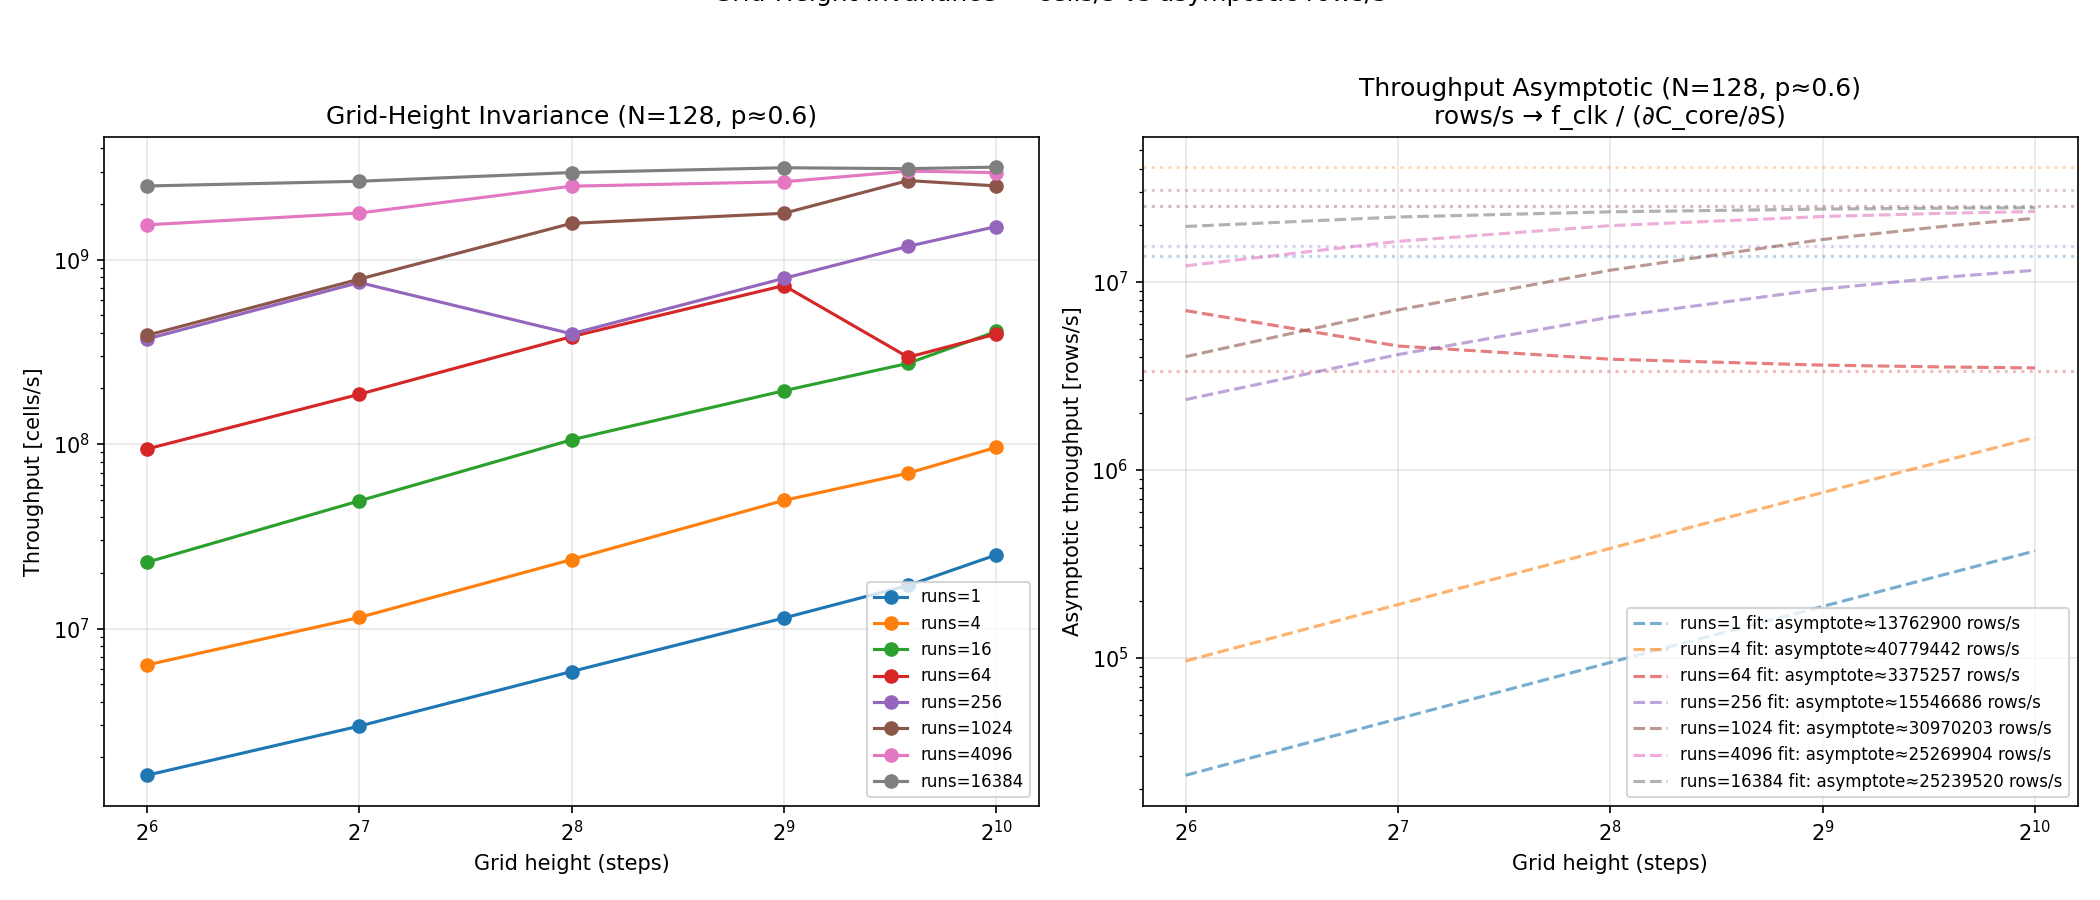
\includegraphics[width=0.6\textwidth]{throughput_invariance.png}\\
    \small Throughput vs grid height
  \vspace{0.3cm}
  \begin{itemize}
    \item Throughput \alert{independent} of grid height (pipeline-dominated)
    \item CV $< 1\%$ across all configurations — FPGA is deterministic
    \item Tiny jitter is entirely host/USB-subsystem noise
  \end{itemize}
\end{frame}

\begin{frame}{Threshold Estimation — Bootstrap}
  \centering
  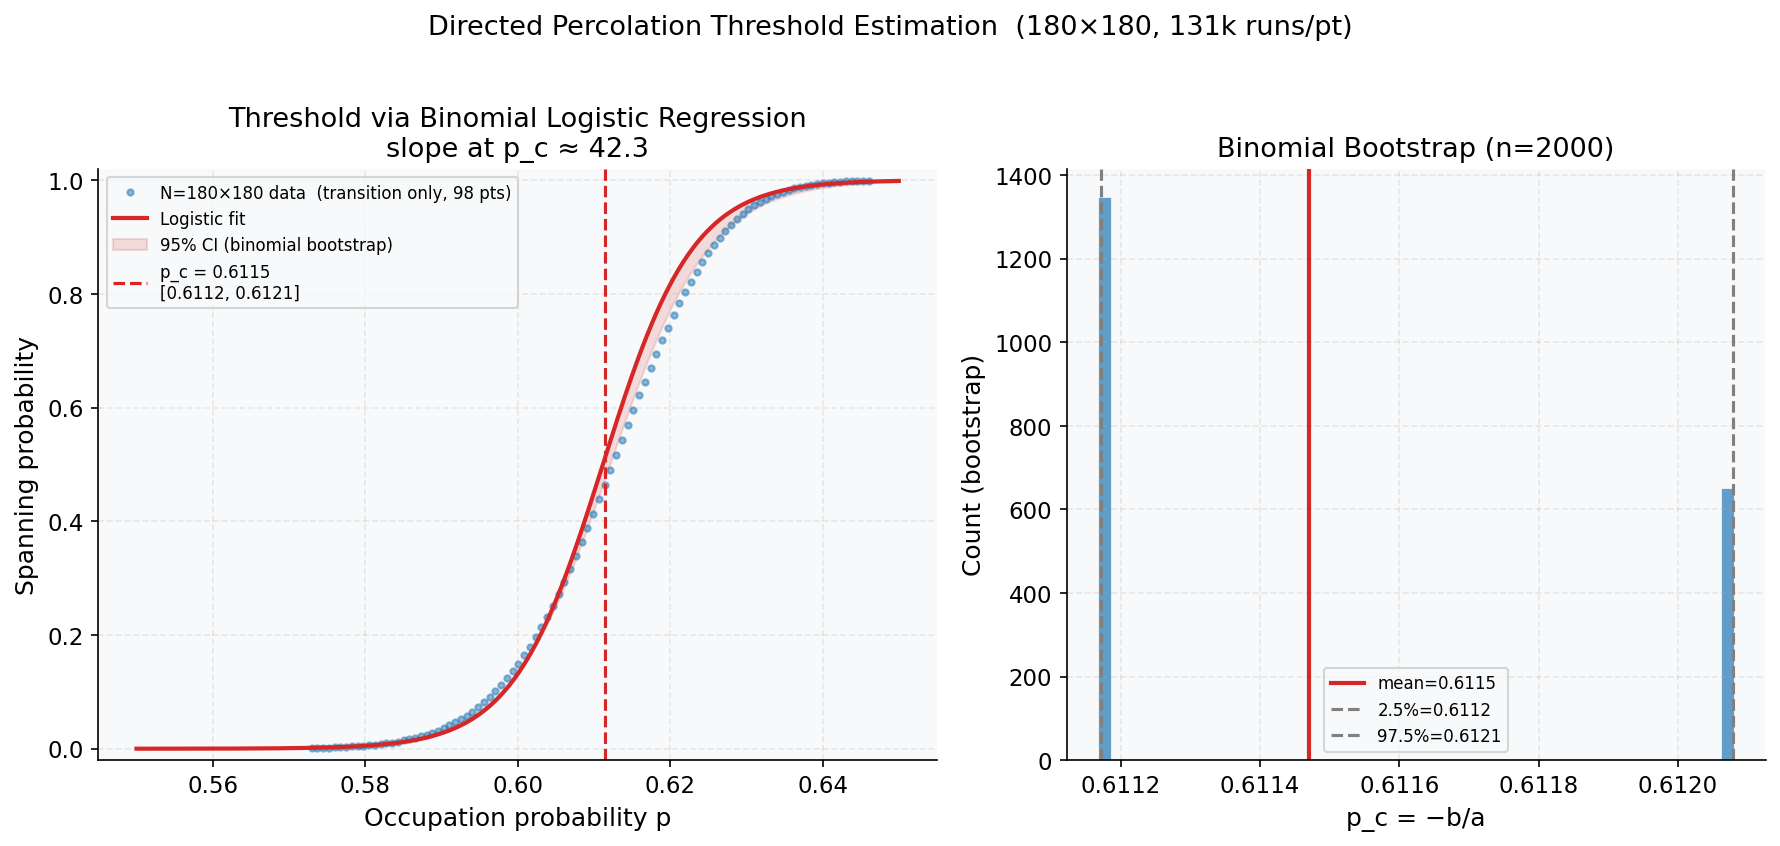
\includegraphics[width=0.75\textwidth]{threshold_bootstrap.png}
\end{frame}

\end{document}
